Submitted:

\begin{verbatim}[1, 3]\end{verbatim}

Chosen option 1 is available?\begin{quote}Yes.\end{quote}Chosen option 3 is available?\begin{quote}Yes.\end{quote}Remarks on your solution:

All given class diagrams are correct?

\begin{quote}\begin{verbatim}No.\end{verbatim}\end{quote}

The correct solution is:\begin{verbatim}[3,4]\end{verbatim}

Your answer to class diagram 1 is not correct.

Class diagram 1 is invalid.

The relationships in the class diagram could be named in the following way:



\begin{centering}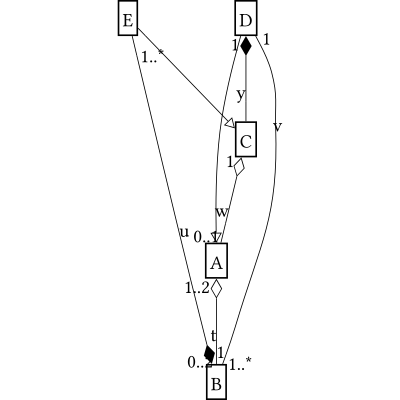
\includegraphics[min width=0.4\textwidth=0.6\textwidth,min height=0.4\textwidth=0.6\textwidth,keepaspectratio,max width=0.9\textwidth,max height=0.9\textwidth]{53/cd304ec9869e94e1ddda9b2aaa917e2b09bc6fc5eb2c530d1213978d80161cb60e01af83b04c596701db35357ce8aed00a3a92e08161.pdf}\end{centering}



If for example composition u would not be there, it would be valid.

Your answer to class diagram 4 is not correct.

Class diagram 4 is valid.

The relationships in the class diagram could be named in the following way:



\begin{centering}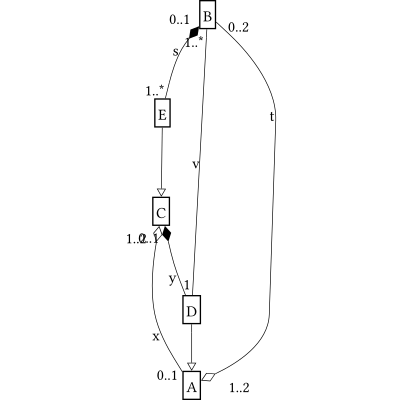
\includegraphics[min width=0.4\textwidth=0.6\textwidth,min height=0.4\textwidth=0.6\textwidth,keepaspectratio,max width=0.9\textwidth,max height=0.9\textwidth]{53/cdf8026e55054824c5b00dbd86a11a47c0e778bb39e7041008f6001317a9eed28f01af83b04c596701db35357ce8aed00a3a92e08161.pdf}\end{centering}



Now consider the following object diagram, which is an instance of this class diagram:



\begin{centering}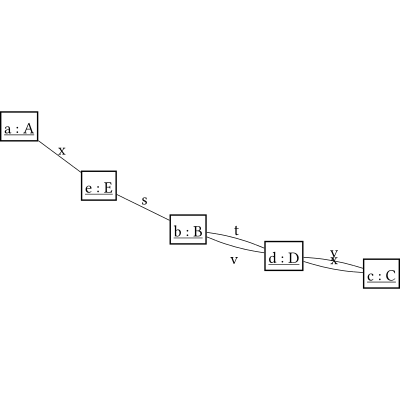
\includegraphics[min width=0.4\textwidth=0.6\textwidth,min height=0.4\textwidth=0.6\textwidth,keepaspectratio,max width=0.9\textwidth,max height=0.9\textwidth]{53/odeb717915f1237f6c1c81d4bbf53a76d1ee08775548a199caba7259f925df238d13.pdf}\end{centering}



